\documentclass[12pt]{report}
% Bibliotheken und Pfade
\usepackage{xcolor} %Farben
\usepackage{graphicx} %Bilder
\usepackage{subfig} %Bilder erweiterung
\usepackage{hyperref} %Links
\usepackage{geometry} %margins
\usepackage[utf8]{inputenc} %Standard!
\usepackage{mathptmx} %Wir benutzen hier eine Mathebibiliothen um Times new Roman zu verwenden
\usepackage[T1]{fontenc} %Standard!
\usepackage{setspace} %zeilenabstände
\usepackage{float}
\usepackage{listings} %code darstellung
\usepackage{blindtext} %Blindtext1
\usepackage{lipsum} %blindtext2
%für deutsch
\usepackage[ngerman]{babel}

\usepackage{titlesec} %zum entfernen der "Kapitel N" header

%wir wollen formatieren{was genau?}[optionaler argument: im block satz.]{kapitel nummerierung und font}{der kapitelname mit angehängtem punkt .}{abstand zwischen nummer und name}{größe titel}
\titleformat{\chapter}[block]{\normalfont\Large\bfseries}{\thechapter.}{1em}{\Large}

\titlespacing*{\chapter}{0pt}{40pt}{30pt} % this alters "before" spacing (the second length argument) to 0
%\titlespacing*{\chapter}{0pt}{50pt}{40pt} % default

\graphicspath{ {images/} }
\geometry{top=3.0cm}


\hypersetup{
    colorlinks,
    linkcolor={black!50!black},
    citecolor={blue!50!black},
    urlcolor={blue!80!black}
}


% Baue die Titel Struktur + Inhalt
\title{
{Bachelorarbeit}\\
{\vspace{10mm}}
{\small Wave-Function-Collapse}\\
{\small Funktionsweise und Anwendungsfälle}\\
{\small TH-Nürnberg Georg-Simon-Ohm}\\
}
% Setze Author und Datum
\author{Davoud Tavakol}
\date{29.12.2022}

% Start Dokument
\begin{document}

% Erstelle den Titel (Dieser Befehlt setzt dann auch den Author und das Datum!)
\maketitle

{\let\clearpage\relax\chapter*{Abstract}}

zum schluss..

% Automatisches Inhaltsverzeichniss
\tableofcontents


%{\let\clearpage\relax\chapter{Abkürzungsverzeichnis}}

%WFC\dotfill{Wave-Function-Collapse}\\
%PCG\dotfill{Procedural-Content-Generation}\\
%CSP\dotfill{Constraint-Satisfaction-Problem}\\

\chapter{Einleitung}

TODO AM ENDE.
Die automatische Generierung von Inhalten wie Texte, Images oder Modellen ist heutzutage Standard in vielen Bereichen der Industrie.
Um solche Inhalte vordefinierten Parametern zu erstellen werden vor allem zwei Methoden zur Generierung verwendend.
AI's {(Künstliche Intelligenzen)} wie ChatGPT und Algorithmen.
Der logische Vorteil von solchen Tools ist es, das diese in kürzester Zeit qualitative Resultate Generieren können und auch wie oben erwähnt vordefinierte Parameter als Input erhalten können,
um die Ergebnisse für ihren gebrauch anzupassen.
In dieser Bachelorarbeit werde ich mich auf den Wave-Function-Collapse Algorithmus, dessen Funktionsweise und Anwendungsfälle fokussieren.

\chapter{Textursynthesen im Vergleich}

Es gibt viele Möglichkeiten Textursynthese mit Algorithmen zu erzielen.
Die meisten dieser Methoden basieren auf demselben Grundprinzip aus kleineren Input-Images größere oder gleich große Output-Images zu generieren.
Nach D.Gomathi und Rajvi Shah {([8], S.1)}, kann die Textursynthese wie folgt definiert werden.\\\\
Ziel einer Textursynthese ist es aus einer Texturprobe eine neue Textur zu generieren die, "wenn sie von einem menschlichen Beobachter wahrgenommen wird,
durch denselben zugrundeliegenden Prozess erzeugt wird."
Das Ergebnis muss der Texturprobe ähnlich sein aber dennoch in der Wahrnehmung genügend Variation enthalten.
So eine Synthese ist nicht möglich, wenn man die Eingabetextur einfach mehrfach kachelt.
Dadurch erhält man keine "sauberen" Übergänge, und die einzelnen Blöcke sind klar erkennbar. {(siehe Abbildung 2.1)}

\begin{figure}[H]
    \centering
    \subfloat[][]{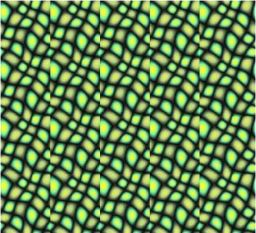
\includegraphics[width=0.4\linewidth]{texture-blocky.JPG}}%
    \qquad
    \subfloat[][]{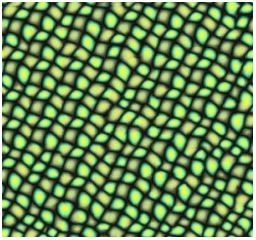
\includegraphics[width=0.4\linewidth]{texture-correct.JPG}}%
    \caption{(a) Blockartige Textur, (b) Textursynthese}%
\end{figure}

\noindent Dadurch ergeben sich folgende Metriken die erfüllt werden müssen.

\begin{itemize}
    \item Wenn Texturprobe gegeben, generiere eine neue Textur, die der Probe gleicht.
    \item Die neue Textur kann eine beliebige Größe haben die vom Benutzer festgelegt wird.
    \item Es sollen keine sichtbaren Übergänge, Artefakte oder fehlerhafte Kanten sichtbar sein.
    \item Dasselbe Muster soll nicht mehrfach in der neuen Textur vorkommen. {([8], S.2)}
\end{itemize}

Im Folgenden werde ich auf drei verschiedene Textursynthese verfahren eingehen da diese sich fundamental voneinander unterscheiden.
Es wird nicht in Detail auf alle verfahren eingegangen da dieser Abschnitt nur Hintergrundinformationen darlegen soll.

\section{Pixel basierende Textursynthese}

Bei dieser Methode werden neue Texturen Pixel für Pixel generiert.
Jeder neue Pixelwert wird von seinen lokalen Nachbarn festgelegt.
Dieser verfahren verwenden meistens Markow-Netzwerke \textit{(Markov-Random-Fields)} die relativ gute Resultate liefern mit wenig Rechenlast.
Markov-Random-Fields Methoden beurteilen jeden Pixel nach einer kleinen Menge von Nachbarn.
Voraussetzung hierfür ist, dass das Input-Image stationär und lokal ist.
Ein Image wird als stationär bezeichnet wenn, unter korrekter Fenstergröße,
jeder betrachtete Bereich ähnlich zueinander aussehen.
Lokal ist ein Image dann, wenn jeder Pixel allein von seinen Nachbarn bestimmt werden kann.{[8]}

\begin{figure}[H]
    \centering
    \subfloat[][]{\includegraphics[width=0.45\linewidth]{Textur-nicht-stationärlokal-2.JPG}}%
    \qquad
    \subfloat[][]{\includegraphics[width=0.45\linewidth]{Textur-stationärlokal-2.JPG}}%
    \caption{(a) Nicht stationär und lokal, (b) stationär und lokal.}%
\end{figure}

Unterschiedliche Bereiche einer Textur sehen sich immer ähnlich {(siehe Abbildung 2.2 (b))}.
Dies ist nicht der Fall für normale Images wie wir bei Abbildung 2.2 {(a)} erkennen können.
Zudem ist es möglich jeden Pixel in {(b)} allein durch seine benachbarten Pixel zu bestimmen.
Diese Attribute bezeichnet man als Stationär und Lokal.{[8]} \\

Funktionsweise eines Algorithmus basierend auf Markov-Random-Fields nach Efros und T. Leung: {[9]}

\begin{figure}[H]
    \centering
    \subfloat[][]{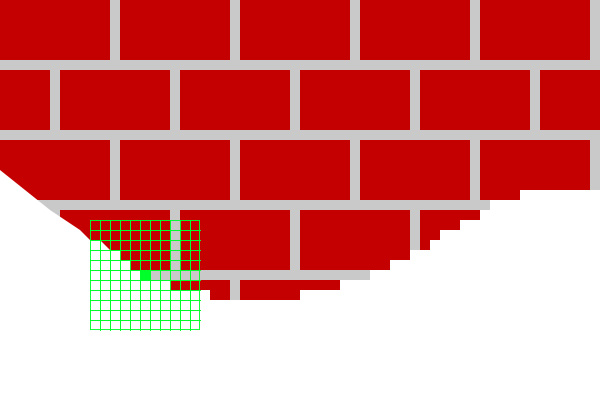
\includegraphics[width=0.45\linewidth]{images/synthezising-pixel.JPG}}%
    \qquad
    \subfloat[][]{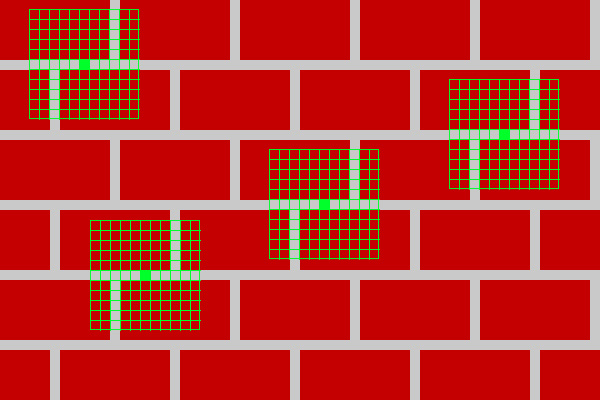
\includegraphics[width=0.45\linewidth]{images/Wall-sample.JPG}}%
    \caption{(a) Pixelsynthese, (b) Sampling des Input-Images.}%
\end{figure}


\begin{itemize}
    \item Zuerst wird vom Input-Image eine Teiltextur einer bestimmten Größe {(z.B. $5\times 5$ Pixel Fenster)} ausgewählt. Von diesem Feld aus werden Spiralförmig neue Pixel generiert.
    \item Für jeden Pixel der betrachtet wird, wird ein Fenster einer selbst bestimmten Größe zentral über das Pixel gelegt.
    Die Größe des Fensters muss nach Größe der einzelnen Elemente der Textur gewählt werden.
    \item Mit dieser Gruppe von Pixel {(der Zentrale Pixel und alle seiner Nachbarn im Fenster)} werden nun alle im Input-Image ähnlichen $N$ Kandidaten gesucht.
    \item Danach wird zufällig von einer dieser Kandidaten ausgewählt und der betrachtete Pixel im Output wird aus diesem Kandidaten kopiert.
    \item Dieser Prozess wiederholt sich so lange, bis alle nicht bekannten Pixel generiert wurden.{([8], S.4)}
\end{itemize}

\section{Pyramid basierende Textur Analyse / Synthese}

Bei der Pyramid-Methode wird das Verfahren der Bildpyramide verwendet.
Hierbei werden aus dem Input-Image mehrere Output-Images in verschiedenen Auflösungen mithilfe von Glättung und Downsampling generiert {(siehe Abbildung 2.4 (a))}. {[8][10]}\\
Zudem wird ein Bildrauschen, \textit{(Noise-Image)} der in der regel uniform Weiß ist, verwendet.
Das Noise-Image wir dann mithilfe von Histogram-Matching und der Image-Pyramid so verändert, das es dem Input-Image ähnlich ist.

\begin{figure}[H]
    \centering
    \subfloat[][]{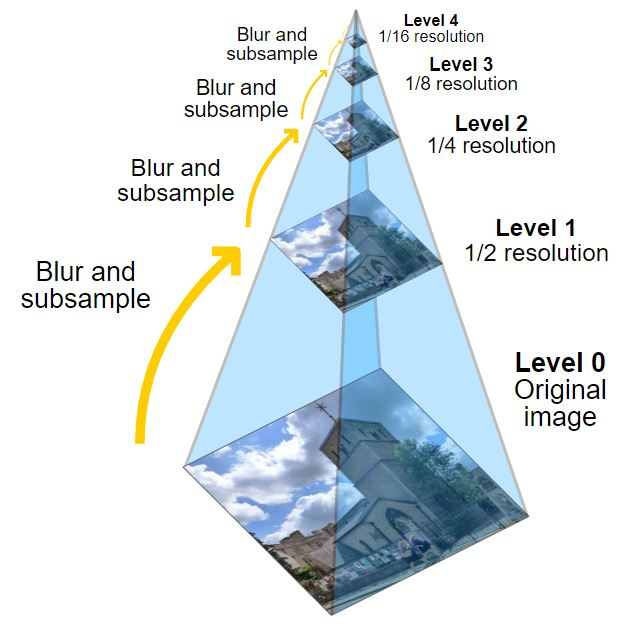
\includegraphics[width=0.4\linewidth]{images/pyramid.JPG}}%
    \caption{(a) Bildpyramide}%
\end{figure}

Histogram-Matching ist die Generalisierung des Punktoperators, mehr spezifisch der Histogrammäqualisation.
Bei der Histogrammäqualisation {(auch Histogrammausgleich, Histogrammeinebnung, Histogrammegalisierung oder Histogrammequalisierung genannt)}
werden die Kontraste von Grauwertbildern derart verbessert, sodass sie über eine bloße Kontrastverstärkung hinausgeht.
Dabei wird die Gleichverteilung mithilfe der Grauwertverteilung berechnet, damit der gesamte zur Verfügung stehende Wertebereich optimal ausgenutzt wird.{[11]}
Bei dem Fall von der Pyramid-Methode nimmt der Algorithmus ein Input-Image und zwingt es über ein Paar von Nachschlagetabellen, ein bestimmtes Histogramm zu haben.
Die beiden Nachschlagetabellen Tabellen sind:

\begin{enumerate}
    \item die kumulative Verteilungsfunktion \textit{(cumulative distribution function (CDF))} eines Bildes und
    \item die inverse kumulative Verteilungsfunktion eines Bildes.
  \end{enumerate}

Die CDF ist eine Nachschlagetabelle, die das Intervall {[0,256]} auf das Intervall {[0,1]} abbildet.
Die inverse CDF ist eine Nachschlagetabelle, die von {[0, 1]} auf {[0, 256]} zurückführt.
Sie wird {(mit linearer Interpolation)} neu abgetastet,
sodass die Stichproben gleichmäßig auf dem Intervall {[0, 1]} verteilt sind.{[8][12]}\\
Während der Algorithmus weiter Iteriert, beginnt das Noise-Image dem Input-Image zu ähneln.
Wir Stoppen die den Prozess, wenn wir eine ausreichende Ähnlichkeit erreicht haben oder wir eine von uns festgelegte Anzahl von Iterationen erreicht haben.

\begin{figure}[H]
    \centering
    \subfloat[][]{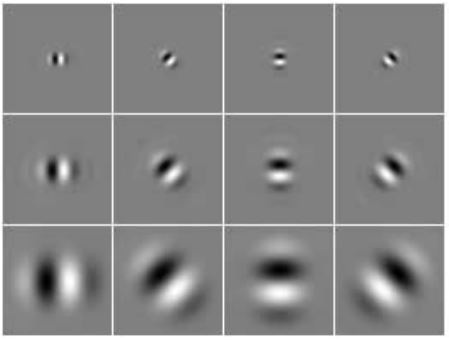
\includegraphics[width=0.2\linewidth]{images/pyramid-noise.JPG}}%
    \qquad
    \subfloat[][]{
\includegraphics[width=0.2\linewidth]{images/pyramid-input.JPG}}%
    \qquad
    \subfloat[][]{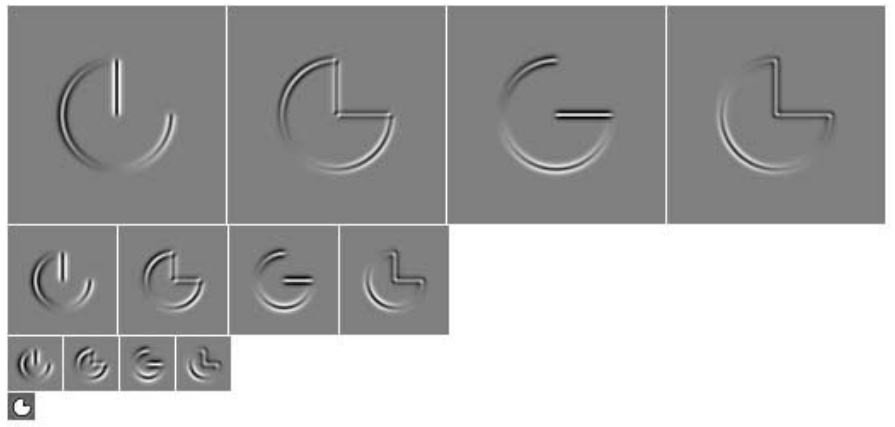
\includegraphics[width=0.3\linewidth]{images/pyramid-matching.JPG}}%
    \caption{(a) Projektion der Bildpyramide, (b) Input-Image, (c) Teilband-Bilder vom Input-Image.}%
\end{figure}

Obwohl die Pyramid-Methode ist im Detail viel komplizierter ist,
werde ich sie hier nicht weiter Behandeln da sie für das weitere Verständnis dieser Arbeit keine Relevanz hat und nur eine weitere Synthesemethode darstellen soll.

\section{Patch basierende Textursynthese}

Die Patch-Based Textursynthese \textit{(auch Quilten genannt)} ist gewissermaßen eine Erweiterung der Pixel basierende Textursynthese.
Hier werden statt einzelne Pixel gleich direkt ganze Felder \textit{(Patches)} verglichen und generiert {(siehe Abbildung 2.6)}.
Auch hier werden die Patches mithilfe ihrer benachbarten Pixel bestimmt und ausgewertet.
Dadruch erhöht sich die Qualität und die Geschwindigkeit des Algorithmus.

\begin{figure}[H]
    \centering
    \subfloat[][]{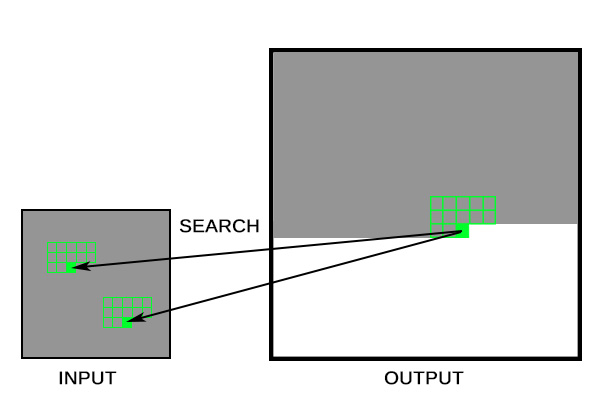
\includegraphics[width=0.45\linewidth]{images/Pixel-based.jpg}}%
    \qquad
    \subfloat[][]{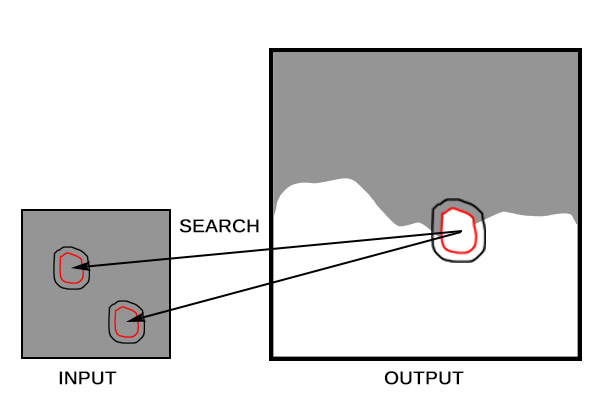
\includegraphics[width=0.45\linewidth]{images/Patch-based.jpg}}%
    \caption{(a) Pixel-Based, (b) Patch-Based.}%
\end{figure}

Ein Problem dieser Synthese im Vergleich zur Pixel-Based Synthese ist, das sich hier die neuen Patches mit bereits vorhandenen Patches überschneiden.
Es gibt viele Methoden, um dieses Problem zu lösen.
Eine davon ist es Patches mit verschiedenen Größen zu verwenden, damit die Konfliktbereiche zwischen den Patches durch das Phänomen der visuellen Maskierung
\textit{(Visual Masking)} reduziert werden.
Gerade bei stationären Texturen erreicht diese Methode gute Ergebnisse.{[8]}

Die Funktionsweise des Algorithmus nach D.Gomathi und Rajvi Shah:

\begin{enumerate}
    \item Generierung des ersten Patches in der oberen-linken Ecke des Output-Images. Der Patch wird zufällig aus dem Input-Image ausgewählt.
    \item Von links-nach-rechts und von oben-nach-unten werden folgende Aufgaben im Output-Image ausgeführt.
    \begin{itemize}
        \item Auswahl des nächsten hinzuzufügenden Feldes aus dem Input-Image aus den am besten passenden Patches.
        \item Berechnen der Fehlerfläche zwischen diesem neuen Patch und seinem Überlappungsbereich mit bereits
        verarbeiteten Patches.
        \item Berechnen des Pfades mit den geringsten Kosten durch die Fehlerfläche, um die Patch grenze zu bestimmen, und fügen Sie dann den neuen Patch zum Output-Image hinzu.
    \end{itemize}
\end{enumerate}

%Images basteln
\begin{figure}[H]
    \centering
    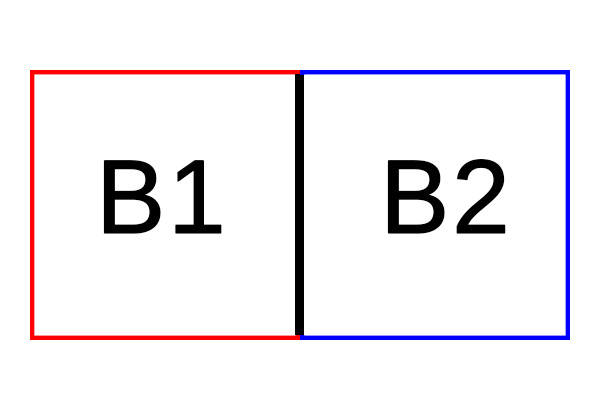
\includegraphics[width=0.25\linewidth]{images/Random-blocks.jpg}%
    \qquad
    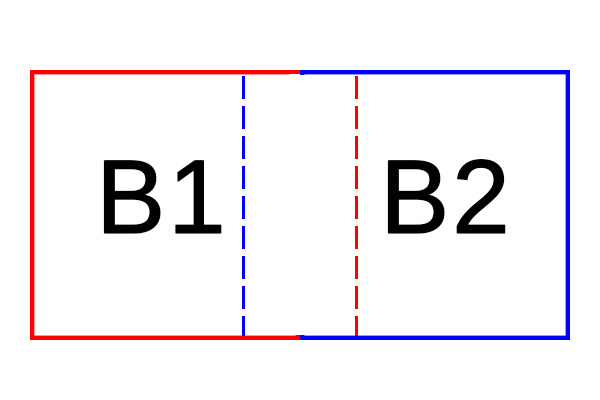
\includegraphics[width=0.25\linewidth]{images/overlap-blocks.jpg}%
    \qquad
    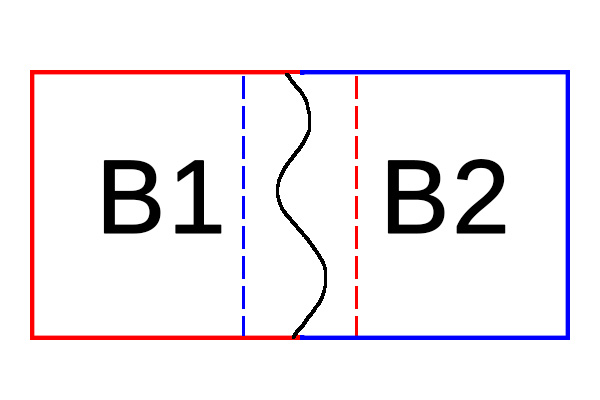
\includegraphics[width=0.25\linewidth]{images/minimum-boundary-blocks.jpg}%
    \qquad
    \qquad
    \subfloat[][]{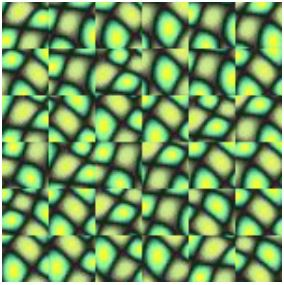
\includegraphics[width=0.25\linewidth]{images/texture-random-block.JPG}}%
    \qquad
    \subfloat[][]{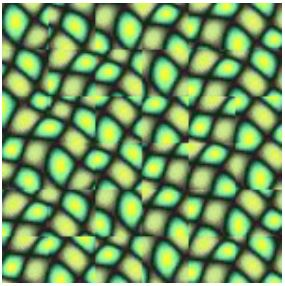
\includegraphics[width=0.25\linewidth]{images/texture-overlap-blocks.jpg}}%
    \qquad
    \subfloat[][]{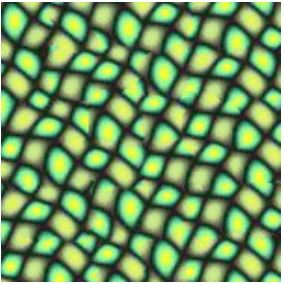
\includegraphics[width=0.25\linewidth]{images/texture-minimum-boundary-blocks.jpg}}%
    \caption{(a) Zufällige Patch Anordnung, (b) Patches eingeschränkt durch Nachbarn, (c) Minimal Fehler Randschnitt. Nach Alexei A. Efros and Thomas K. Leung. [9]}%
\end{figure}

\chapter{Wave-Function-Collapse}

Wichtig bei allen Textursynthesen ist,
das die Muster des Output-Images immer lokal ähnlich oder gleich dem des Input-Images sind.
Das wird größtenteils dadurch erzielt das aus dem Input-Image kleinere Subimages, Patches oder Pixel extrahiert werden.
Bei den verfahren, wo die lokale Ähnlichkeit nicht 1-zu-1 bzw. pixelgenau stattfindet, werden die Pixel und deren Farbwert oft nach Grundlage der Abstandsmetrik {(z.B. dem euklidischen Abstand von Pixelfarbvektoren)} beurteilt.
Solche Verfahren finden meistens in der rein visuellen Computergrafik Anwendung.
Diese Methodiken haben große Nachteile im Gegensatz zu Algorithmen wo das lokale Muster des Outputs pixelgenau dem Input-Image gleicht.
Gerade bei PCG {(Procedural-Content-Generation)} kann die Pixelgenauigkeit von großen Nutzen sein da dadurch Abgrenzungen der Pixel innerhalb des Output-Images klar definiert sein können. {[1]}
Von allen oben beschriebenen Textursynthese Methoden ist WFC wahrscheinlich der Patch-Based Methode am ähnlichsten.\\

Gumin hat sich von der Arbeit von Paul Merrell Inspirieren lassen, obwohl dieser sich Hauptsächlich mit der Generierung von 3D-Modellen befasst hatte.
Bei seinem Verfahren werden die Modelle mithilfe von bereits erstellten Bausteinen zusammengesetzt.
Das ist dahingehen wichtig da in vielen Textursynthesen gerade bei den Übergängen die Pixel sich Mischen und somit sich Artefakte bilden können.
Dieser Verhalten ist bei WFC und dem Verfahren von Paul Merrell nicht möglich da es sich um eine diskrete Synthese handelt.
Jedes lokale Muster ist immer im Input wiederzufinden {(siehe Abbildung 3.1)}. {[1][3][4]}

\begin{figure}[H]
    \centering
    \subfloat[][]{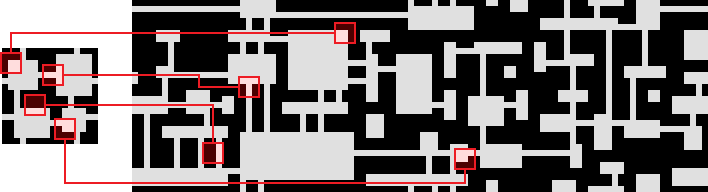
\includegraphics[width=1\linewidth]{images/wfc-pattern.png}}%
    \caption{(a) WFC generiertes Muster.}%
\end{figure}

\section{Constraint-Satisfaction-Problem}

Der WFC von Gumin ist lose an der Quantenmechanik angelehnt.
Das liegt daran, dass bei der Synthese von WFC in jeder Zelle des $N\times N$ Output-Images theoretisch jedes Muster / Pixelwert vorkommen kann bevor sie final festgelegt werden.
Dieser Zustand nennt sich \textit{Superposition}.
Jede Zelle hat mehrere Eigenwerte \textit{(eigenstates)} und somit auch eine maximale Entropie bzw. einen maximalen Informationsgehalt.
Auch hat jede Zelle bestimmte Regeln, bestimmt durch ihre Nachbarn, die erfüllt werden müssen.
Denn nicht jede Zelle kann an jeder Position auftauchen, sobald bereits eine Zelle ein Eigenwert erhält.
{(Siehe Patch-Based Textursynthese. Nicht jeder Patch kann an einer beliebigen Position sein.
Sie müssen sich schließlich an den Nachbarn anpassen damit die Synthese nahtlos ist.)}
Sobald eine Zelle bekannt wird \textit{(Observation)} und damit nur einen Eigenwert besitzt,
dann wird die Entropie aller anderen Zellen angepasst. {[2]}
Da der WFC Algorithmus genau auf diese Art und Weise seine Synthese durchführt,
dann kann man den WFC auch als Löser für solche Bedingungserfüllungsprobleme \textit{(Constraint-Satisfaction-Problem)} verwenden.\\

\subsection{Was ist ein Constraint-Satisfaction-Problem {(CSP)}?}

Grundsätzlich beschreiben CSP's Gruppen von Objekten denen Variablen zugeteilt sind.
Diesen Variablen sind Regeln, sogenannte \textit{(constraints)}, auferlegt die erfüllt werden müssen.
Jeder dieser Variablen hat zu Beginn eine Superposition und kann damit jeden wert enthalten.
Die Aufgabe von Algorithmen zum Lösen von CSP's \textit{(solver)} ist es einen Zustand \textit{(State)} zu finden in denen alle constraints erfüllt sind und jeder Variable nur noch ein wert zugeordnet ist.
Für solche Probleme finden sich oft bei der Künstlichen Intelligenz und aus dem Operations Research. {[5]}
Im Fall von WFC sind die Objekte, denen die Variablen zugeteilt sind, die einzelnen Bereiche im Output-Image.
Jeder diese Bereiche muss ein lokales Muster aus dem Input zugeordnet werden.
Immer, wenn einem Bereich ein wert zugeordnet wird, dann werden auch die benachbarten Bereiche damit beeinflusst \textit{(Propagation)}.
Der Gesamtprozess, wenn sich eine Gruppe aus Superpositionen mit mehreren Eigenwerten zu einem einzelnen Eigenwert aufgrund von Interaktion mit der Außenwelt \textit{(Observation)} reduziert,
nennt sich Wave-Function-Collapse. {[6]}
Während dem Prozess einen gültigen State für das CSP zu finden, dann gibt es immer Situationen in dem es mehrere gültige Optionen für eine Variable gibt.
Wenn so eine Situation auftritt, dann haben verschiedene Solver verschiedene Ansätze.
Einige Algorithmen wähle zufällig eine der möglichen Werte von momentan zulässigen Optionen.
Bei so einem Ansatz kann es sein das der Algorithmus nicht auf einen Zustand kommen kann, in dem alle constraints erfüllt werden können.
In so einem Fall gibt es Rücksetzverfahren \textit{(Backtracking)} bei dem der Algorithmus zu seinem letzten Ergebnis zurückfällt und ein anderen Wert für die Variable setzt, um aus dem
ungültigen Zustand zu kommen.
Andere Algorithmen verwenden zusätzliche Heuristiken abgesehen von den bereits bekannten constraints, um die Möglichkeit eines ungültigen Zustandes zu reduzieren. {[1]}

\subsection{CSP-Beispiel an Sudoku}

Es gibt viele verschiedene CSP Probleme.
Eines der bekanntesten Probleme, welchen viele Menschen schon fast täglich selbst lösen, ist Sudoku.
Sudoku ist ein CSP welcher am besten auch die Funktionsweise von Gumins WFC aufzeigt, da die Constraints der Probleme sehr ähnlich sein können.\\\\
Wenn wir ein Sudoku Feld ohne initiale Zahlen betrachten \textit{(unobserved)}, dann kann in jedem einzelnen Feld theoretisch jede Zahl vorhanden sein \textit{(Superposition)}.

\begin{figure}[H]
    \centering
    \subfloat[][]{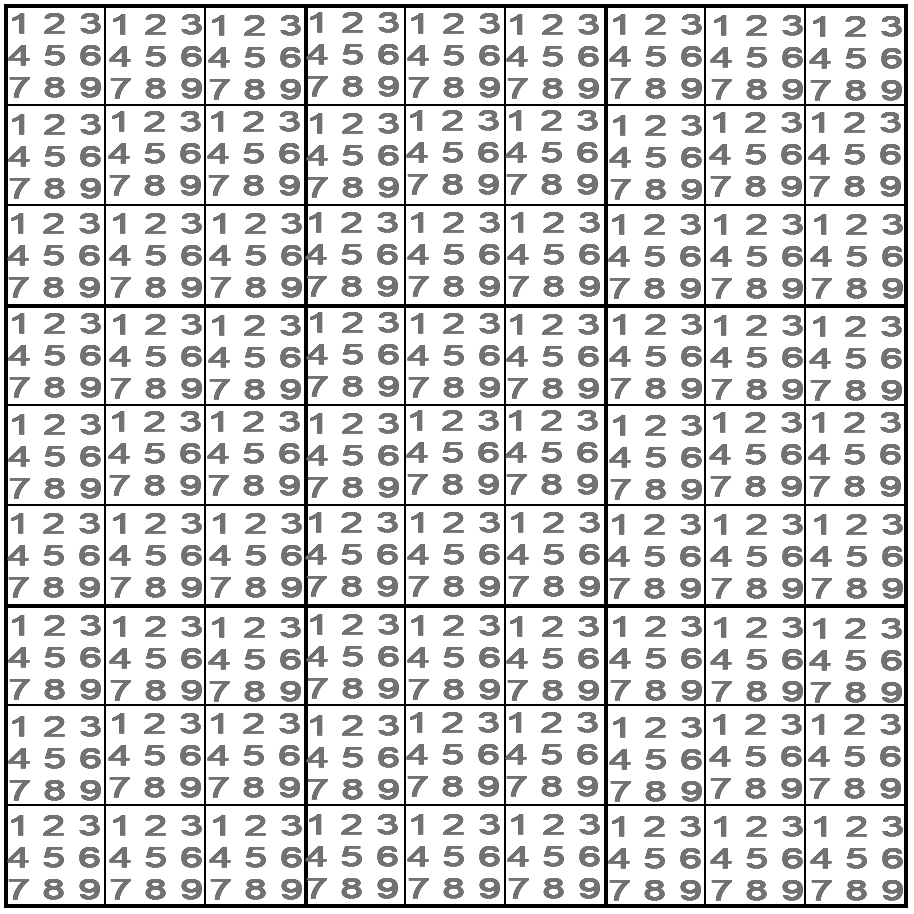
\includegraphics[width=0.9\linewidth]{images/sudoku-superposition.png}}%
    \caption{(a) Sudoku Feld unbeobachtet in einer Superposition.}%
\end{figure}

Die Regeln \textit{(constraints)} dieses CPS sind wie folgt:
\begin{enumerate}
    \item Jede Zeile, Spalte und jedes Quadrat {(je 9 Felder)} muss mit den Zahlen 1-9 ausgefüllt werden.
    \item Keine Zahl innerhalb der Zeile, Spalte oder des Quadrats darf sich wiederholen.
\end{enumerate}

Der nächste Schritt ist die \textit{Observation}, sprich das erste Feld mit seinen vielen Eigenwerten einen festen wert Zuordnen.
Dadurch treten für die benachbarten die Constraints ein, die bestimmen welche Werte sie nun noch einnehmen können.

\begin{figure}[H]
    \centering
    \subfloat[][]{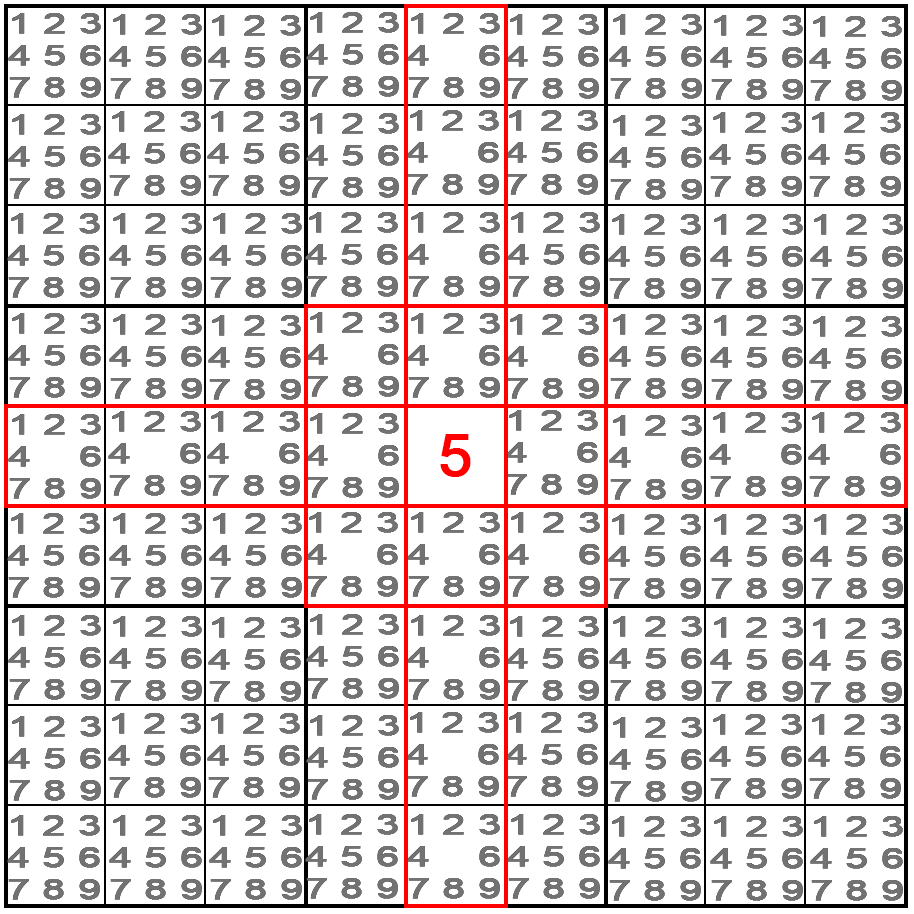
\includegraphics[width=0.9\linewidth]{images/sudoku-observed.png}}%
    \caption{(a) Sudoku Feld mit dem ersten Input.}%
\end{figure}

Nach dem ersten Input reduziert sich die Entropie aller Zellen in jeder betroffenen Zeile,
Spalte und Quadrat bzw. ihre Anzahl an möglichen Eigenwerten reduziert sich.
Als nächsten Schritt könnte man jetzt eine beliebige Zelle auswählen und diese auf einen Zufälligen möglichen Eigenwert setzten.
Allerdings besteht so immer die Möglichkeit, dass der Prozess an einen Punkt kommt, an dem kein gültiger Zustand erreicht werden kann.
Um dieses Szenario unwahrscheinlicher zu machen {(aber immer noch möglich!)} können wir uns Heuristiken zu nutzen machen,
um eine Auswahl zu treffend die uns wahrscheinlicher zu einem gültigen Endzustand bringt.
In diesem Fall können wir uns eine Zelle aussuchen die Bereits eine sehr niedrige Anzahl an möglichen Eigenwerten hat.
Dadurch ist die Chance geringer das wir eine Zelle auf einen ungünstigen Wert setzten, der später zu einem ungültigen Endzustand führt.
{(Achtung! Dies ist nicht zwingend der fall für WFC. Dazu später mehr.)}

\begin{figure}[H]
    \centering
    \subfloat[][]{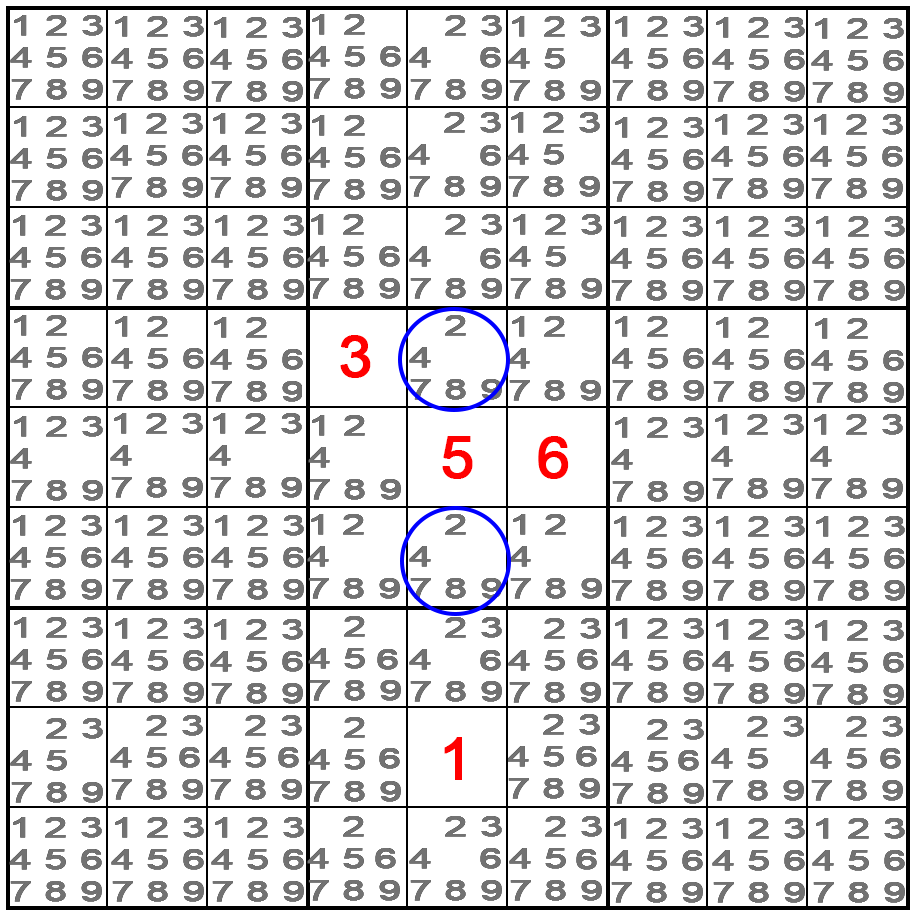
\includegraphics[width=0.9\linewidth]{images/sudoku-observed-heurisitk.png}}%
    \caption{(a) Sudoku Feld mit mehreren festgelegten Zellen. Blau markierte Zellen sind mögliche Kandidaten für nächsten Zyklus.}%
\end{figure}

Dieser Zyklus wiederholt sich so lange, bis alle Zellen ausgefüllt sind.

\section{WFC und die Model Synthese}

Wir hatten bereits erwähnt das Gumins Wave-Function-Collapse Algorithmus von Paul Merrell's diskreter Model Synthese inspiriert ist.
Die Model Synthese hingegen ist nicht nur ein Löser für CSP's wie WFC, sondern ebenfalls auch von der Patch-Based Synthese inspiriert.
Textursynthese funktionierte im Allgemeinen relativ gut in vielen Bereichen.
Allerdings taten sich einige Synthesen schwer damit, mit festen Strukturen als Input zu arbeiten, als auch Objekte im 3D-Raum zu generieren.
Diese Probleme wollte Paul Merrell mit seiner Model Synthese lösen.

\begin{figure}[H]
    \centering
    \subfloat[][]{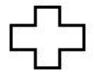
\includegraphics[width=0.1\linewidth]{images/input-shape.JPG}}%
    \qquad
    \subfloat[][]{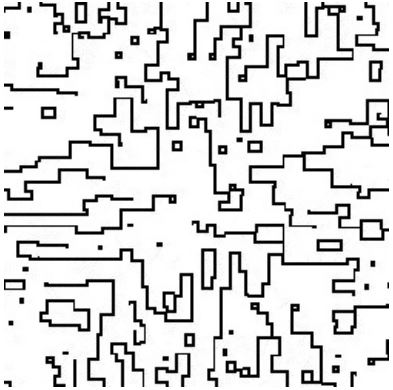
\includegraphics[width=0.25\linewidth]{images/Efros-Leung-1999.JPG}}%
    \qquad
    \subfloat[][]{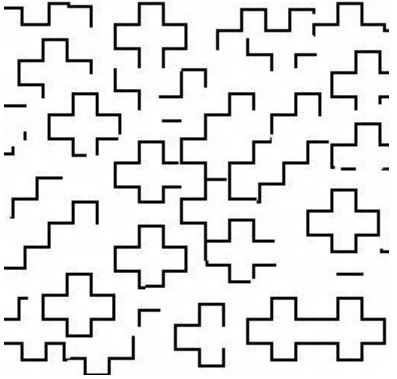
\includegraphics[width=0.25\linewidth]{images/Kwatra-2005.JPG}}%
    \caption{(a) Input Struktur, (b) Alexei A. Efros and Thomas K. Leung 1999, (c) Kwatra et al., 2005. [3]}%
\end{figure}

In Abbildung 3.5 können wir klar die Schwachstellen von anderen Textursynthesen erkennen.\\
Paul Merrell erkannte das viele natürliche und künstliche Objekte aus sich immer wiederholenden Komponenten bestehen.
Deswegen kam er auf die Idee, anstatt mit einzelnen Pixel, lieber mit ganzen Komponenten zu Arbeiten.
Dadurch konnte er neue Objekte sowohl in 2D als auch in 3D-Raum generieren.

\begin{figure}[H]
    \centering
    \subfloat[][]{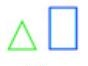
\includegraphics[width=0.1\linewidth]{images/Beispiel-textur.JPG}}%
    \qquad
    \subfloat[][]{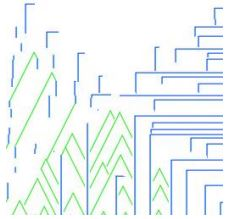
\includegraphics[width=0.25\linewidth]{images/Efros-Leung-textur.JPG}}%
    \qquad
    \subfloat[][]{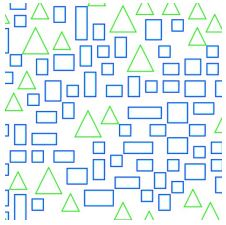
\includegraphics[width=0.25\linewidth]{images/Paul-merrells-Model-synthese.JPG}}%
    \caption{(a) Input Struktur, (b) Alexei A. Efros and Thomas K. Leung, (c) Paul Merrell Model Synthese. [3]}%
\end{figure}

Anders als bei Sudoku, gibt es hier die Regel der Adjazenz-Bedingung \textit{(adjacency constraint)}.
Die Adjazenz-Bedingung stellt sicher, dass alle Teile des Modells nahtlos zusammenpassen und dass das neue Modell dem Input ähnelt.

\begin{figure}[H]
    \centering
    \subfloat[][]{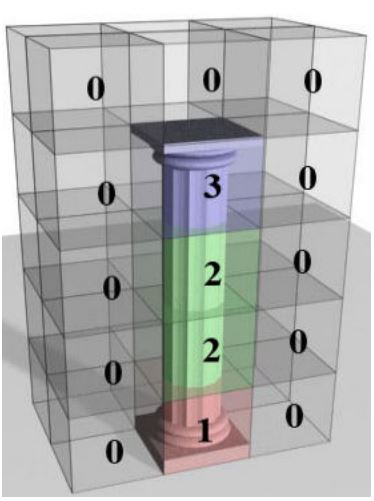
\includegraphics[width=0.1\linewidth]{images/model-divided.JPG}}%
    \qquad
    \subfloat[][]{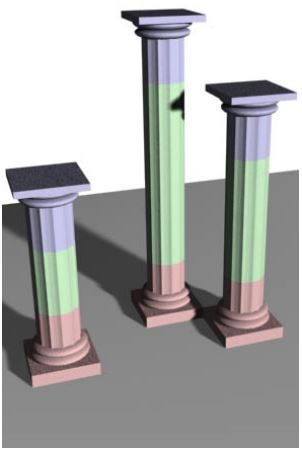
\includegraphics[width=0.25\linewidth]{images/seamless-model.JPG}}%
    \qquad
    \subfloat[][]{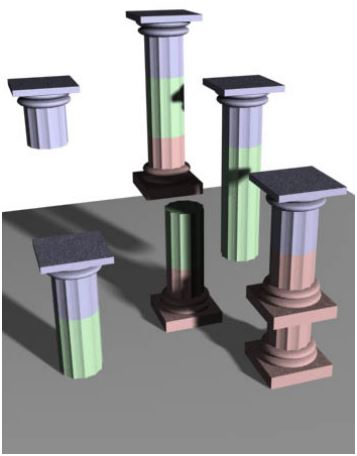
\includegraphics[width=0.25\linewidth]{images/modell-conflicts.JPG}}%
    \caption{(a) 3D-Modell in Komponenten aufgeteilt, (b) Komponente nahtlos zusammengesetzt, (c) Komponente halten Adjazenz-Bedingung nicht ein. [3]}%
\end{figure}

Der Grundsätzliche ablauf der Model Synthese, im 2D-Raum, ist wie folgt:

\begin{enumerate}
    \item Erstelle Module.
    \begin{figure}[H]
        \centering
        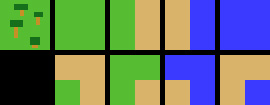
\includegraphics[width=0.4\linewidth]{images/modules-cells.JPG}
    \end{figure}
    \item Wähle Zelle unter eventueller Berücksichtigung von Heuristiken.
    \item Kollabiere Zelle auf einen Eigenwert.
    \item Errechne neue mögliche Eigenwerte der benachbarten Zellen \textit{(Propagation)}.
    \begin{figure}[H]
        \centering
        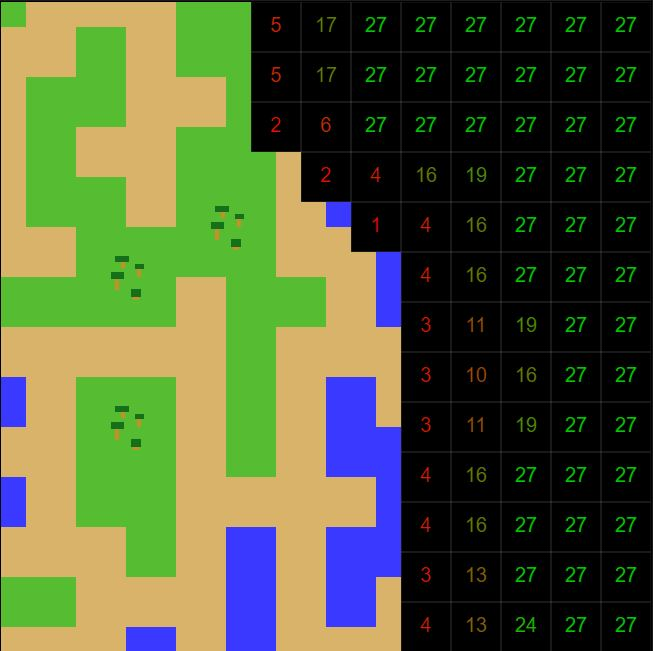
\includegraphics[width=0.6\linewidth]{images/collapse-cells.JPG}
    \end{figure}
    \item Wiederhole Schritte 2 - 4.
\end{enumerate}

An diesem Punkt ist es wichtig zu erwähnen,
dass es sich hierbei bereits um die \glqq Simple Tile Model\grqq{} des WFC Algorithmus handelt.

\subsection{Unterschiede zwischen WFC und Model Synthese}

Tatsächlich ist der WFC Algorithmus von Gumin und die Model Synthese von Merrell, in der Ausführung der oben genannten Schritte, exakt derselbe Algorithmus.

Der Unterschied zwischen den beiden Algorithmen besteht lediglich in der Implementierung der einzelnen Schritte sowie in zusätzlichen Optimierungen,
die die Model Synthese im Vergleich zu WFC besitzt.
Laut Paul Merrell gibt es mehrere Unterschiede in der Implementierung.\\
Eine davon ist die Reihenfolge der Auswahl der nächsten Zelle.
Während WFC nach der niedrigsten Entropie Heuristik seine Zelle auswählt,
wählt die Model Synthese nach der Scanline-Methode, in der erst Reihe für Reihe durch das Modell / Bild iteriert wird, seine Zelle aus.
Interessanterweise verursacht die Zellenauswahl von WFC mehr Fehlerzustände bei großen Output-Images.
Auch die Komplexität des Inputs kann dazu beitragen das WFC nicht zu einem Ergebnis kommt, während das bei der Model Synthese wesentlich unwahrscheinlicher ist.\\
Ein weiterer Grund warum die Model Synthese gerade bei großen Modellen wesentlich öfter zu Ergebnissen kommt, ist die Blockweise Generierung vom Output-Image.
In Paul Merrells Model Synthese wird der Output Blockweise generiert und nicht komplett in einem Durchgang.
Das ist für die Generierung von großen Outputs, vor allem bei 3D-Modellen, von großer Bedeutung da dadurch die Fehlerquote bei einigen Inputs signifikant reduziert wird.
WFC teilt sein CSP nicht in kleinere Blöcke auf, da der Output von WFC in der Regel kleiner ist, und die Verarbeitung im 2D-Raum wesentlich einfacher.
Das bedeutet nicht das WFC von so einer Implementierung nicht profitieren würde, vor allem wenn man WFC im 3D-Raum verwenden möchte.
Jedoch kann ab diesen Punkt einfach die Model Synthese verwendend werden. {[13]}

\begin{figure}[H]
    \centering
    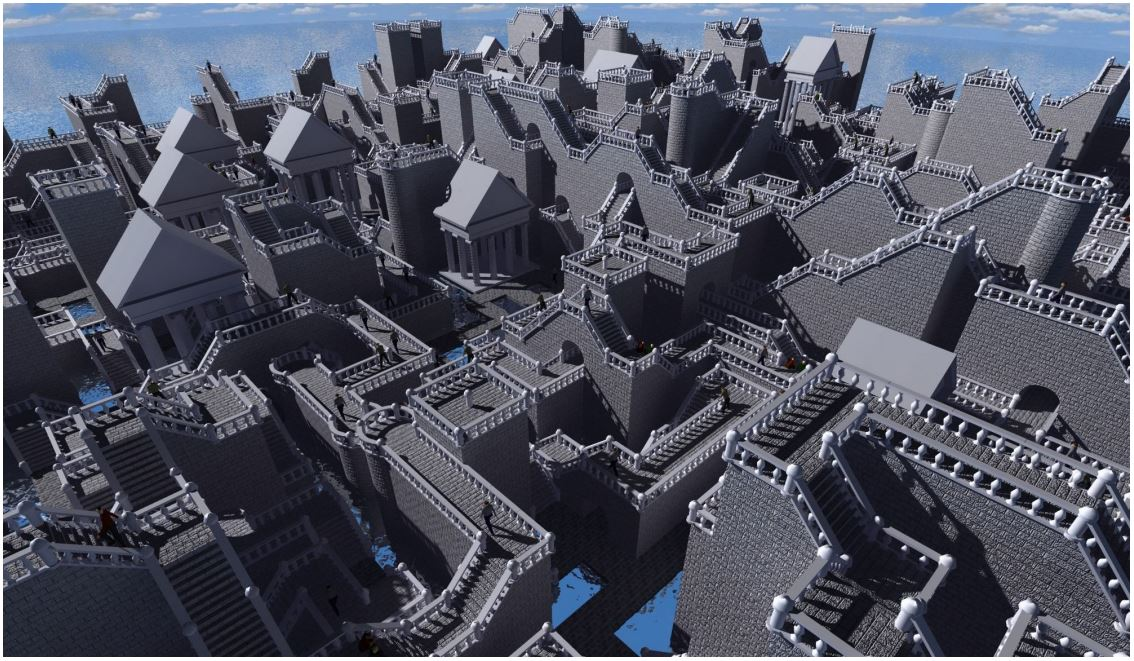
\includegraphics[width=1\linewidth]{images/3D-model-synthese.JPG}%
    \caption{3D-Modell generiert mit Model Synthese.}%
\end{figure}

Neben weiteren Unterschieden wie die Laufzeit und der Erweiterbarkeit der beiden Algorithmen so gibt es noch einen weiteren Unterschied den WFC implementiert.
Das sogenannte Overlapping Model von WFC, das in der Originalversion von Gumin vorkommt, ist das, was WFC initial so bekannt gemacht hat.

\subsection{Simple Tile Model und Overlapping Model}

Anders als bei der Simple Tile Model von WFC, wo die einzelnen Module / Patches für die Synthese einzeln bereitgestellt werden,
benötigt das Overlapping Model von WFC ein komplettes Input-Image welches Analysiert wird.
Aus dieser Analyse werden die Module automatisch generiert.
Zudem haben sich die Patches bei der Simple Tile Model nicht überschnitten was bei dem Overlapping Model, offensichtlich, der Fall ist.
Das hat den Vorteil das die Patches ganz einfach aus dem Input errechnet werden können und der Output sieht dem Input ähnlicher da die Patches enger aneinander liegen. {[13]}

\begin{figure}[H]
    \centering
    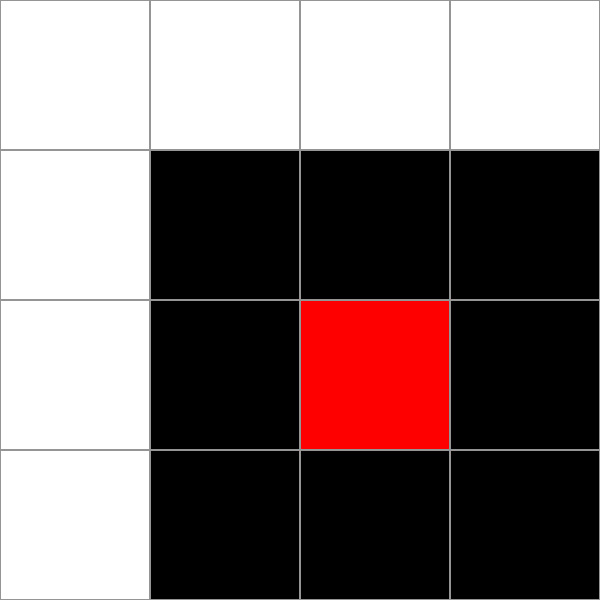
\includegraphics[width=0.5\linewidth]{images/red-maze.jpg}%
    \caption{$4\times 4$ Pixel Red-Maze Beispiel Input.}%
\end{figure}


\begin{figure}[H]
    \centering
    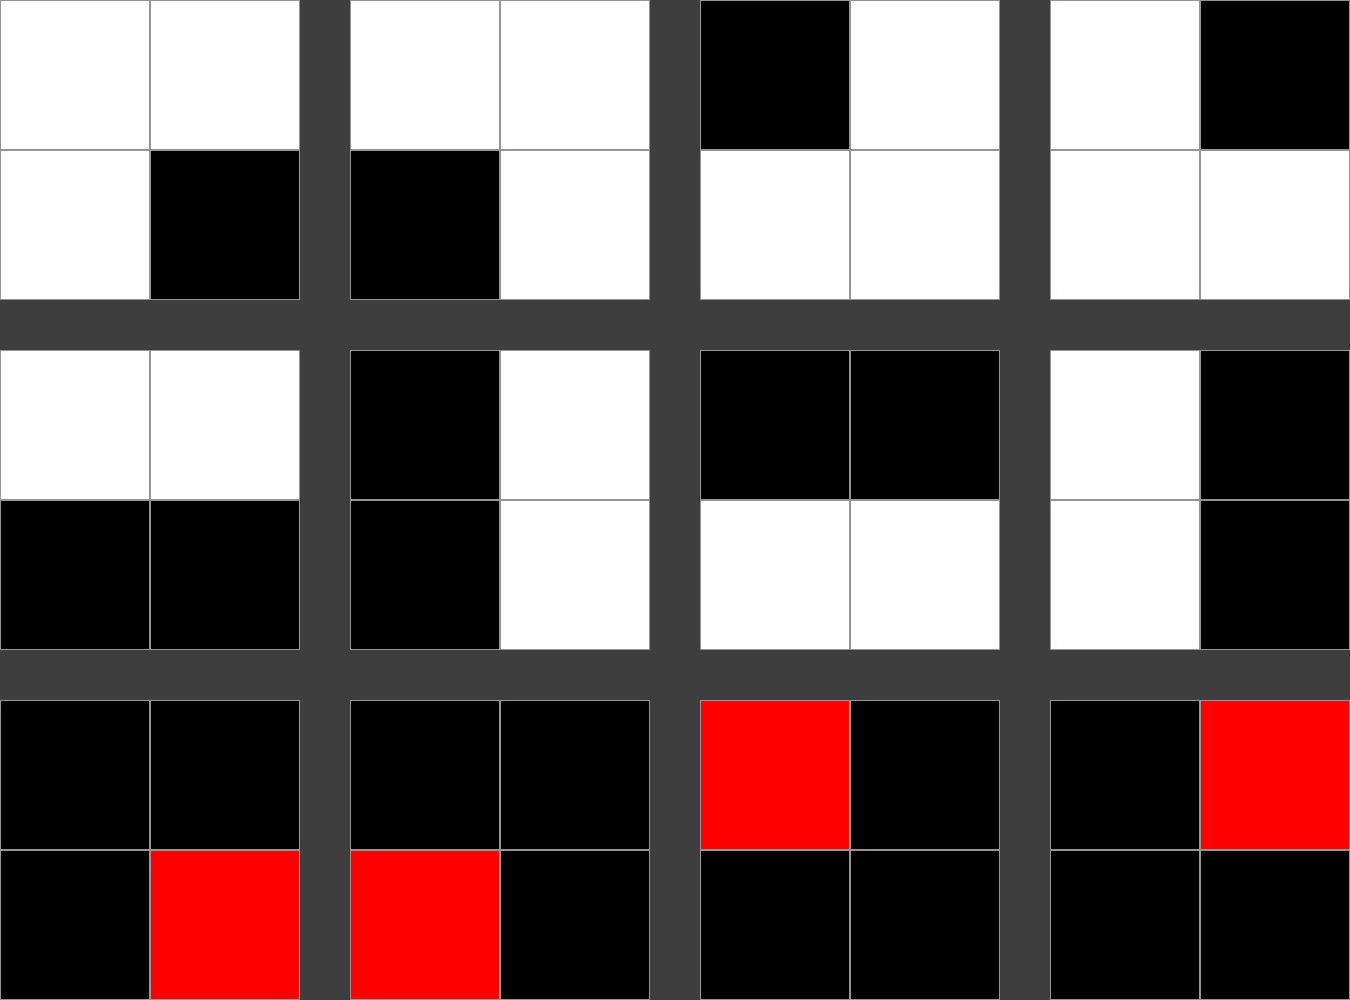
\includegraphics[width=0.5\linewidth]{images/red-maze-modules.jpg}%
    \caption{Alle Red-Maze Module der Größe $N = 2$ mit Spiegelungen und Rotationen.}%
\end{figure}

Bei einem $N = 2$ Patch gibt es insgesamt 9 verschiedene Möglichkeiten wie diese übereinander liegen können.
{(Wenn $N = 3$ dann $(2(N - 1) + 1)^2 = 36$ offsets.)}
Der WFC Algorithmus legt eine Indexstruktur an, die die Möglichkeiten beschriebt, wie ein die Muster nebeneinander platziert werden können.
Bei diesem Model enthält der Index die vorberechnete Anzahl an gültigen Patches, die an einem anderen Index mit $x,y$-Offset platziert werden darf. 
Man kann sich vorstellen das jede Zelle im Sudoku Feld ein bestimmte $x,y$ Koordinate besitzt damit durch diese Iteriert werden kann.
Sobald ein Feld einen Wert besitzt, dann werden in allen benachbarten Zellen die Patches entfernt, die nicht nutzbar sind. {[1]}

\begin{figure}[H]
    \centering
    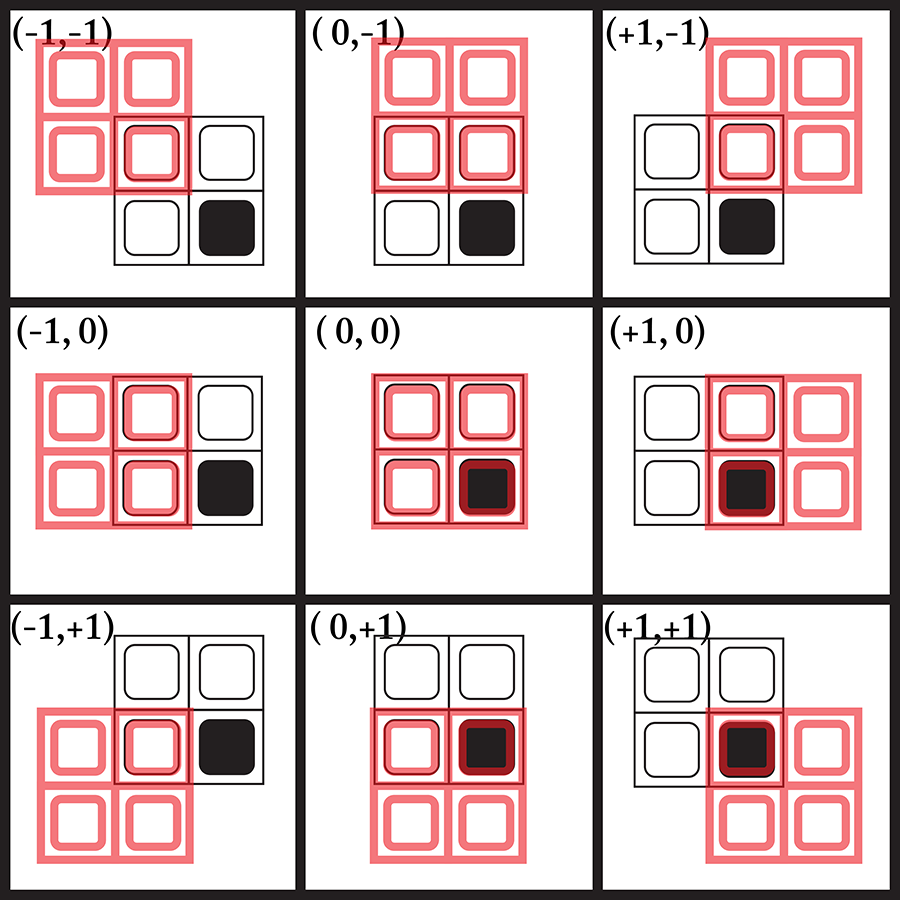
\includegraphics[width=0.5\linewidth]{images/red-maze-offset.png}%
    \caption{Die 9 Möglichkeiten wie die Patches übereinander liegen können.}%
\end{figure}

In Abbildung 3.12 sehen wir einen Ausschnitt einer einzelnen Zelle mit allen möglichen Patches die an seinen benachbarten $x,y$-Offsets erlaubt sind.
Angemerkt sei das bei offset $(0,0)$ {(kein Offset)} immer nur ein möglicher Patch nutzbar ist, der betrachtete Patch {(bzw. die Zelle mit bereits einzelnem Eigenwert)} selbst.
{(Siehe z.B. Offset $(-1,0)$. Dort sind nur Patches möglich die Rechts 2 weiße Pixel besitzen damit sie sich nahtlos mit den 2 weißen Pixel bei $(0,0)$ überlappen können)}{[1]}

\begin{figure}[H]
    \centering
    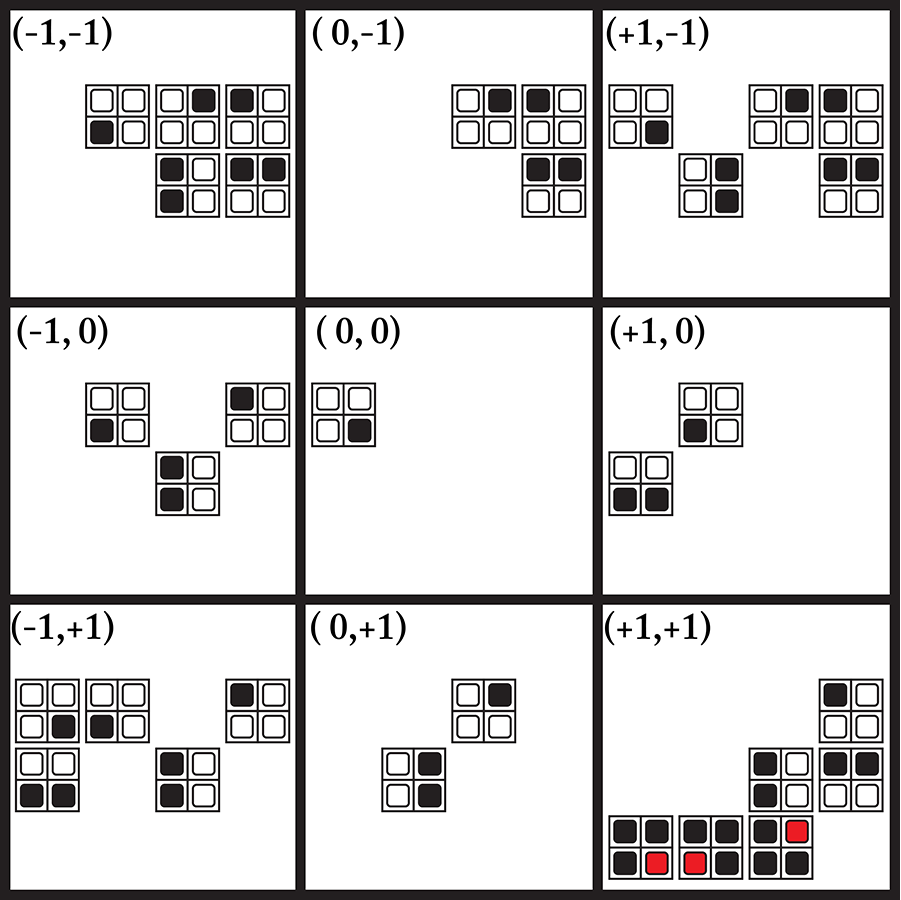
\includegraphics[width=0.5\linewidth]{images/red-maze-offset-example.png}%
    \caption{Ausschnitt einer Zelle. Von 12 möglichen Patches sind nur die gültigen Optionen für die benachbarten Zellen mit $x,y$-Offset möglich.}%
\end{figure}

In diesem Beispiel wurden mit $N = 2$, also eine Fenstergröße von 2 Pixel, die Module aus dem Input generiert.
Die Fenstergröße wir selbst von Entwickler festgelegt und hat direkten Einfluss auf den Output.
Falls $N = 1$ festgelegt wird dann befinden wir uns wieder beim Simple Tile Model.
Allerdings funktioniert $N = 1$ in diesem Fall nicht, da jeder Pixel zu einem "Patch" wird die wir diese selbstverständlich nicht mehr überlappen können.
Bei zu kleiner Fenstergröße kann der Output nicht dem Input ähneln.
Andersrum bei einer zu großen Fenstergröße kann der Output dem Input zu ähnlich sein.
Man muss aufpassen welche Größe man wählt, um ein gewünschtes Ergebnis zu erhalten.

\begin{figure}[H]
    \centering
    \frame{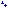
\includegraphics[width=0.25\linewidth]{images/input-example-overlapping.png}}%
    \caption{Beispiel Input-Image ($8\times8$ Pixel) für Overlapping Model}%
\end{figure}

\begin{figure}[H]
    \centering
    \subfloat[][]{\frame{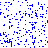
\includegraphics[width=0.25\linewidth]{images/output-overlapping-n2.png}}}%
    \qquad
    \subfloat[][]{\frame{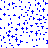
\includegraphics[width=0.25\linewidth]{images/output-overlapping-n3.png}}}%
    \qquad
    \subfloat[][]{\frame{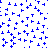
\includegraphics[width=0.25\linewidth]{images/output-overlapping-n4.png}}}%
    \caption{(a) Output mit $N = 2$, (b) Output mit $N = 3$, (c) Output mit $N = 4$. Beispiele generiert mit Kchapelier's Overlapping Model [14]}%
\end{figure}

Es ist wichtig anzumerken das viele der hier gezeigten Texturen auch mit aktuellen Textursynthese-Algorithmen generiert werden können.
Der Vorteil von Model Synthese und WFC im Vergleich zu anderen Synthesen ist das der generierte Content auch Interaktiv genutzt werden kann,
da wir vollen Kontrolle über die lokalen Muster des Outputs haben.
Gerade der Simple Tile Model bietet sich deswegen für Procedural-Content-Generation {(PCG)} an, da wir hier auch volle Kontrolle über die einzelnen Module / Patches haben,
dann zusammengesetzt werden für den Output.
Dadurch bietet sich WFC gerade für die Spiele-Entwicklung an, da dadurch keine unvorhersehbaren Artefakte entstehen können.
Andersrum hingegen wenn statt einem lokalen und stationären {(siehe Abbildung 2.2)} Input ein Foto verwendet wird,
dann würden die anderen Synthesemethoden passendere Ergebnisse liefern im Gegensatz zur Model Synthese und WFC.
Es sei erwähnt das der Input für WFC nicht \glqq strikt\grqq{} eine Textur wie in Abbildung 2.2 {(b)} sein muss.
Sie sollte allerdings Selbstähnlichkeit besitzen und nur wenige unterschiedliche Pixelfarben verwenden.\\
Bereits ein Tag nach der Veröffentlichung von Gumin's WFC am 30. September 2016 haben viele Entwickler bereits begonnen mit diesem Algorithmus zu experimentieren.
Grund für die große Beliebtheit dafür ist nicht nur die bereits erwähnten Pixelgenauigkeit und die damit einhergehende Möglichkeit den Output Interaktiv zu nutzen,
sondern auch die live Generierung des Outputs selbst.
Viele PCG's Methoden variieren in ihrer Laufzeit bei der Generierung ihres Outputs.
Dies führt dazu das manchmal bereits Großteile des Outputs sofort generiert werden,
dafür aber der Abschluss aufgrund von komplexen constraint solving Algorithmen nicht gleichmäßig entsteht. {[1]}
Da WFC nach der niedrigsten Entropie Heuristik seine nächste Zelle auswählt und im Overlapping Model alle benachbarten Zellen, die nicht kollabiert sind,
alle möglichen Pixelwerte enthält, dann führt das zu einer sehr schön anzusehenden Generierung des Outputs.

\begin{figure}[H]
    \centering
    \frame{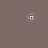
\includegraphics[width=0.4\linewidth]{images/red-maze-overlapping-step1.png}}%
    \caption{
        Resultat des ersten Zyklus mit dem Red-Maze Input. Da am Anfang die Entropie überall gleich ist, wird die Anfangszelle zufällig gewählt.
        Da der Algorithmus bereits die möglichen Patches der benachbarten Zellen ausgewertet hat, werden die Zellen mit allen verwendbaren Patches eingefärbt.
        {(Die Pixelfarben werden dann gemischt)}.
        Dadurch ist der Bereich direkt um der Anfangszelle nicht in einer einheitlichen Farbe dargestellt, da es dort bereits weniger Optionen gibt die verwendet werden können.
        {(Siehe Abbildung 4.12)} {[1]}.
    }%
\end{figure}

\begin{figure}[H]
    \centering
    \frame{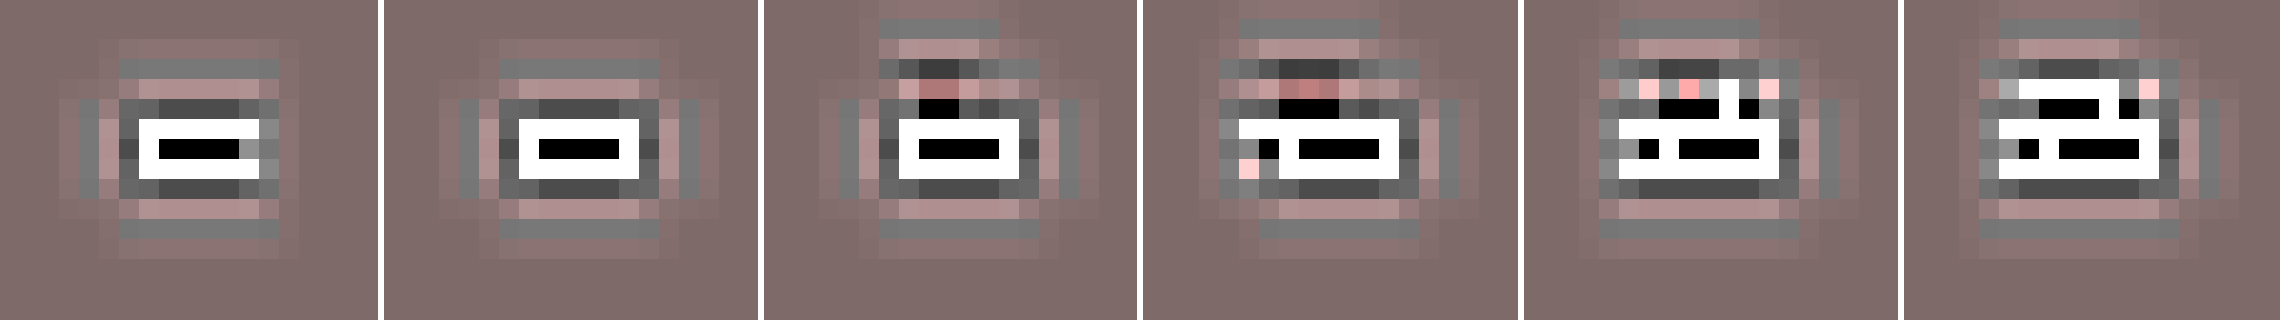
\includegraphics[width=1\linewidth]{images/red-maze-overlapping-steps.png}}%
    \caption{Die nächsten Zyklen für das Red-Maze Input. {[1]}}%
\end{figure}

\section{Beispiel Implementierung}

Joseph Parker war einer der ersten, die WFC verwendet haben.
In seinem \textit{Proc Skater 2016} [15] verwendete er den Algorithmus in Unity um einzigartige 3D Skateparks zu generieren.
Er verwendete selbst erstellte Blöcke, aus denen die Karten generiert werden sollen, anstatt sie automatisch aus einem Input zu analysieren.
Trotzdem benutze er den Overlapping Ansatz zum Platzieren der einzelnen Blöcke, um saubere Übergänge zu garantieren.

\begin{figure}[H]
    \centering
    \frame{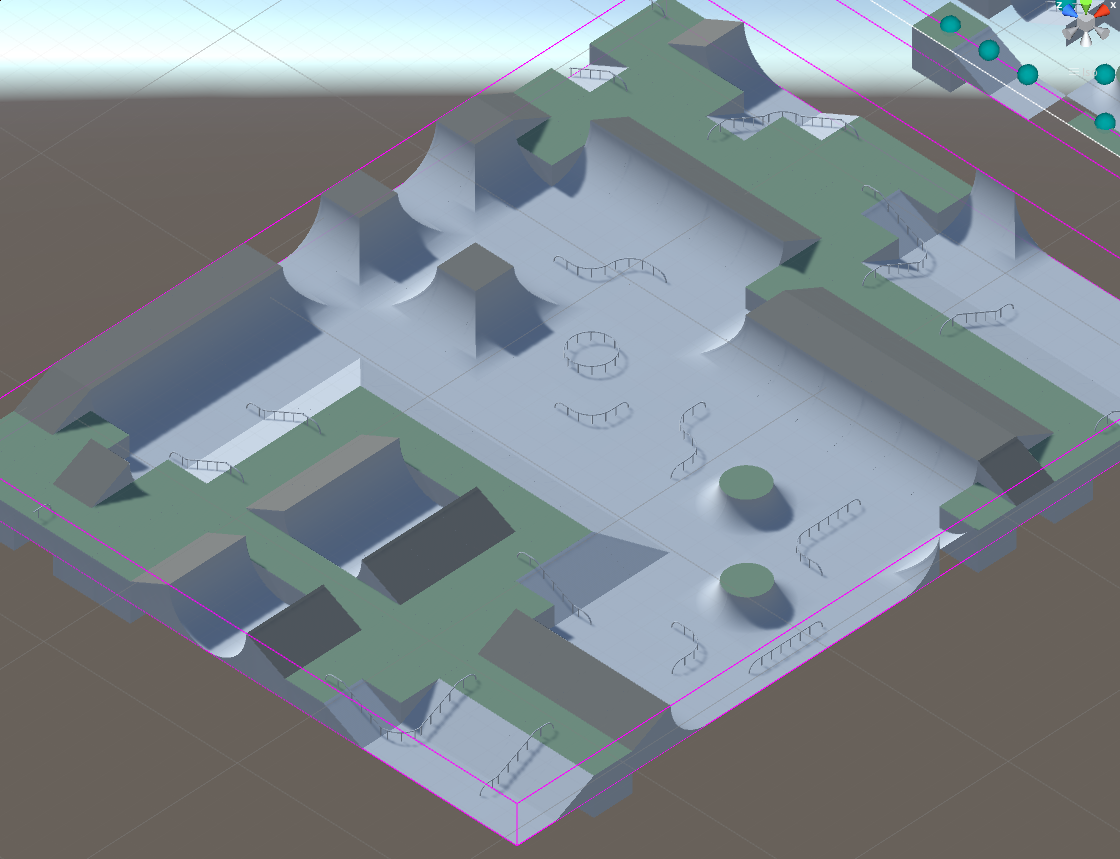
\includegraphics[width=1\linewidth]{images/proc-skater.png}}%
    \caption{Level generierung in \textit{Proc Skater 2016.} {[15]}}%
\end{figure}

Eine weitere kommerzielle Implementierung von WFC ist \textit{Caves of Qud}, entwickelt von Freehold Games.
Laut Brian Bucklew, einem der Entwickler bei Freehold Games, verwendet \textit{Caves of Qud} ein Mehrfachdurchlauf \textit{multipass} von WFC.
Dadruch können größere Komplexitäten bei der Generierung erreicht werden.
Ein weiterer Vorteil, der sich dadurch ergeben hat, ist die einfache Handhabung von WFC.
Sobald das zugrundeliegende System vorhanden ist, kann jeder Entwickler einfach Input-Images einspielen und Spielbaren Content generieren.{[1][16]}

\begin{figure}[H]
    \centering
    \frame{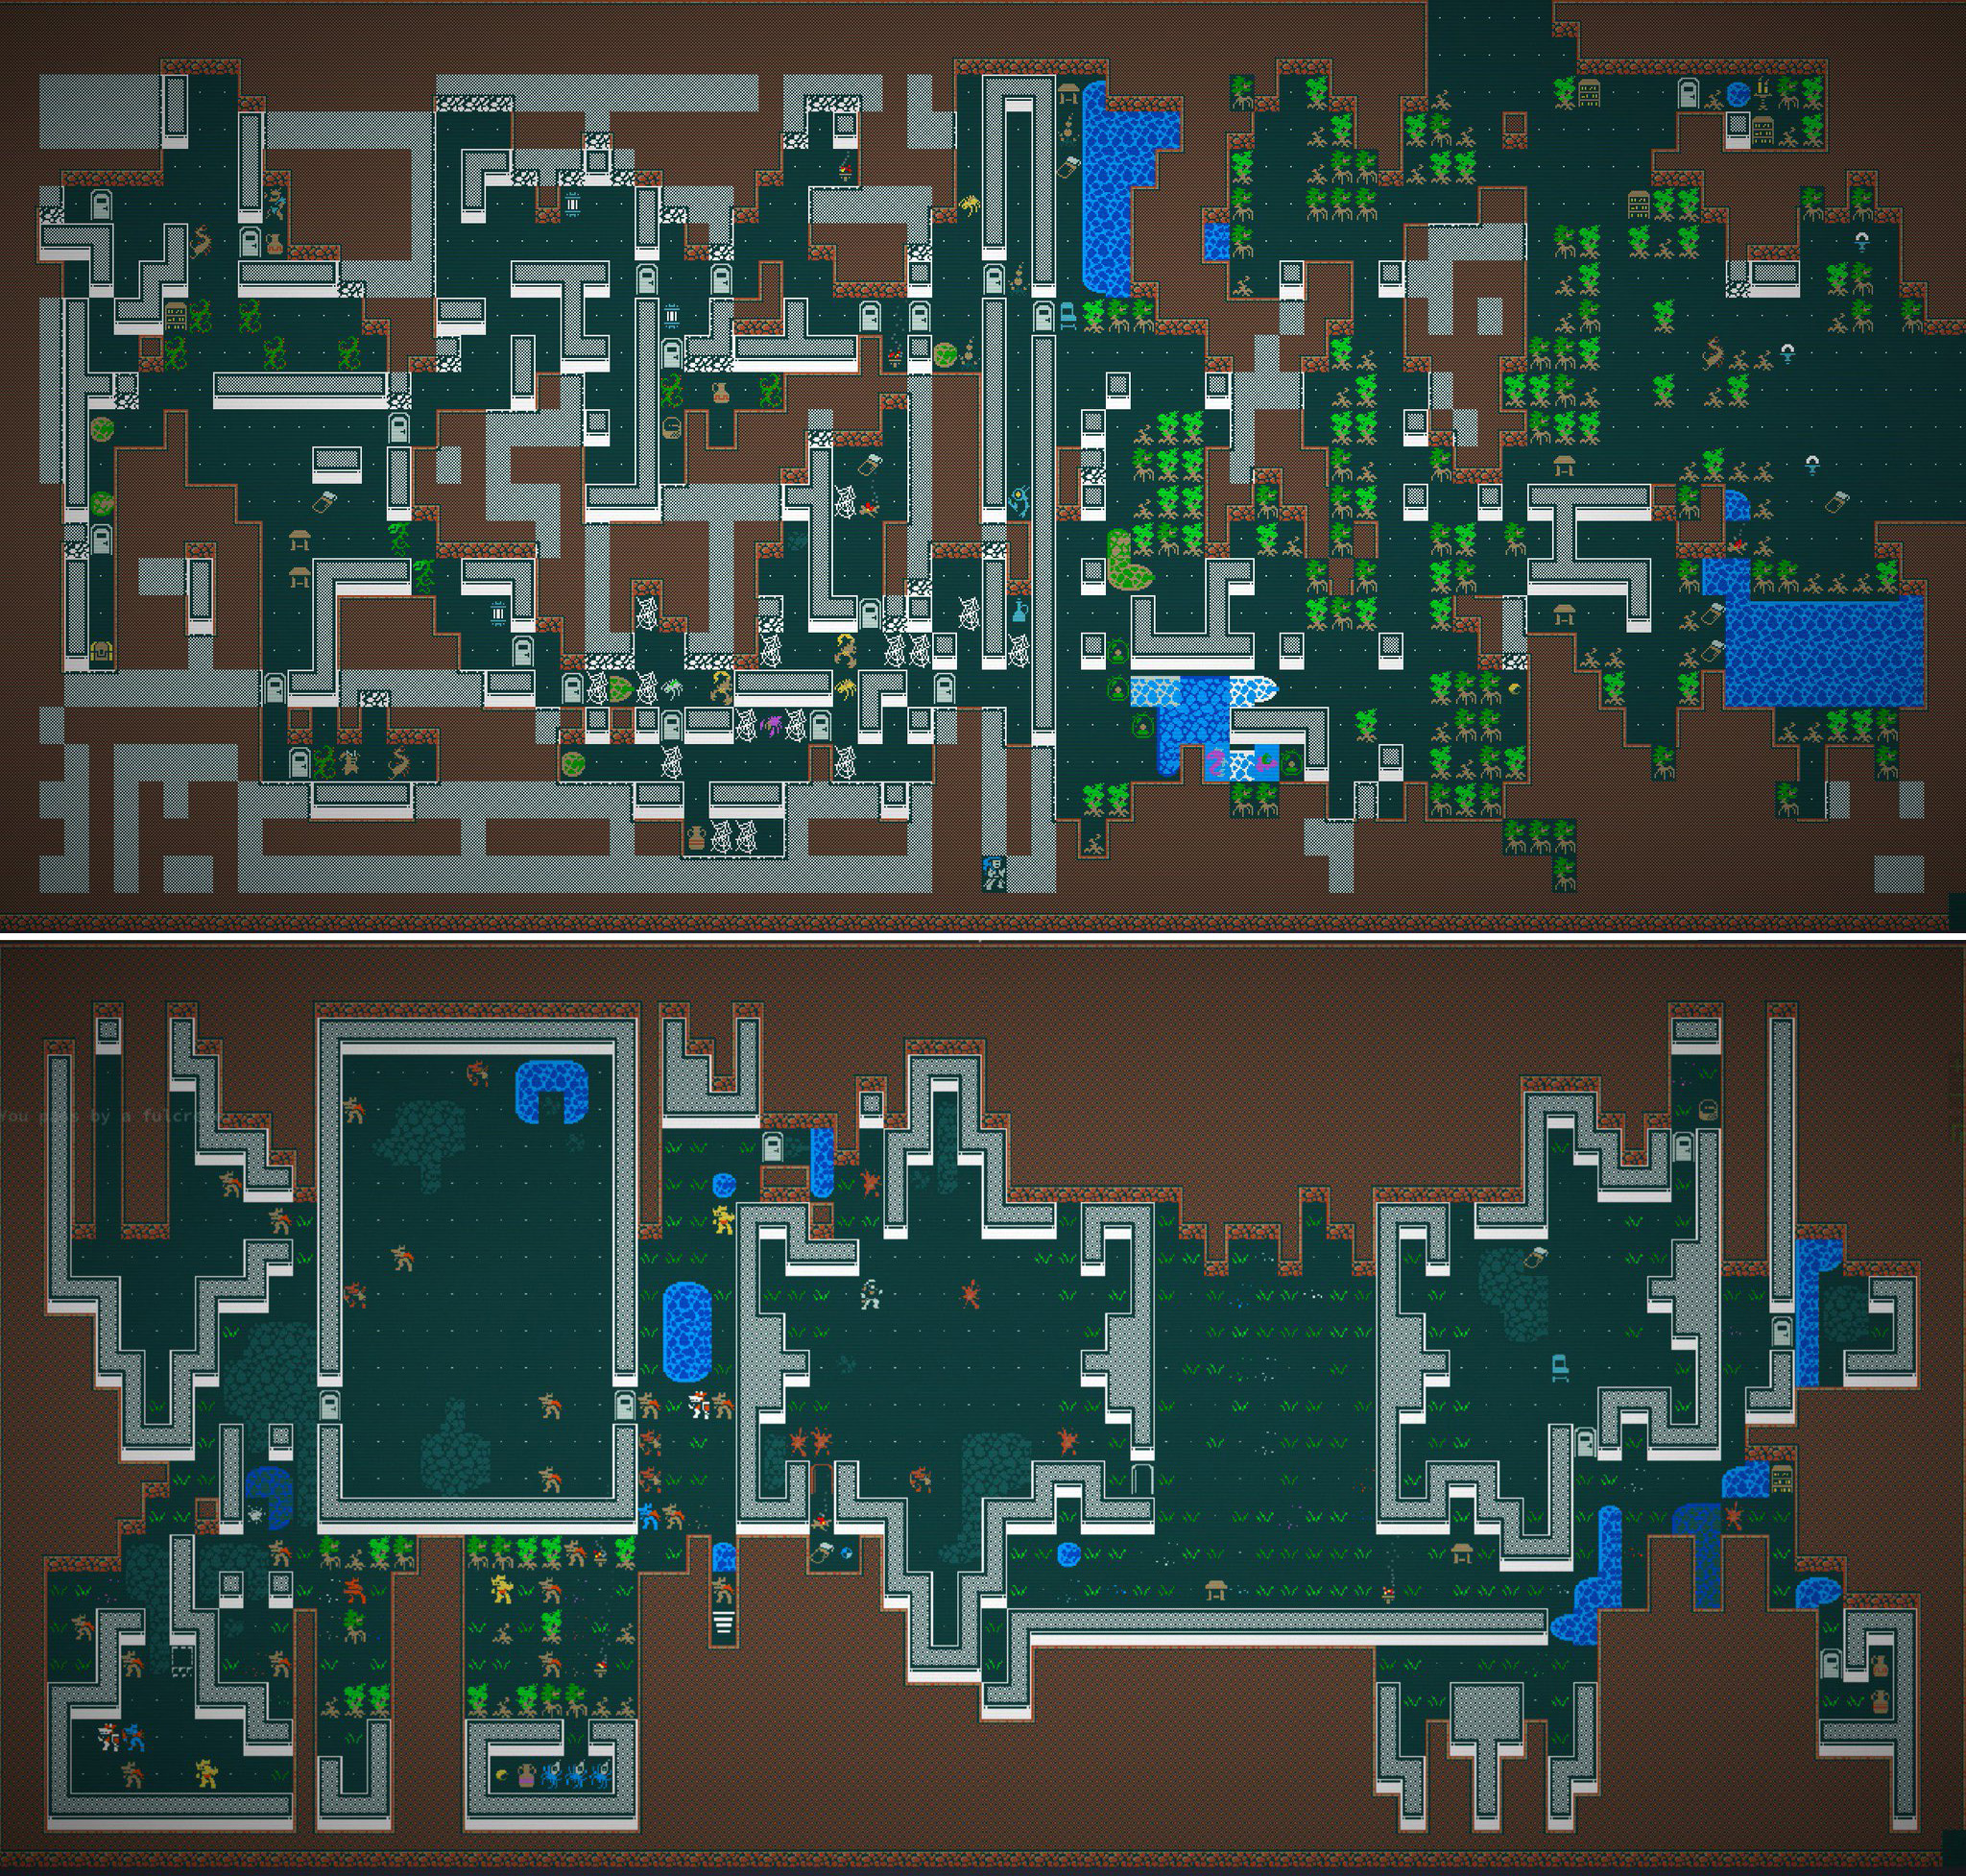
\includegraphics[width=1\linewidth]{images/caves-of-qud.png}}%
    \caption{Zwei Spielbare Karten von \textit{Caves of Qud.} {[1][16]}}%
\end{figure}

Wave-Function-Collapse kann nicht nur auf Planaren ebenen mit quadratischen zellen verwenden werden...

{\let\clearpage\relax\chapter{Fazit}}

{\let\clearpage\relax\chapter{Literaturverzeichnis}}
{[1]} \url{https://adamsmith.as/papers/wfc_is_constraint_solving_in_the_wild.pdf}\\
{[2]} \url{https://en.wikipedia.org/wiki/Wave_function_collapse}\\
{[3]} \url{https://paulmerrell.org/wp-content/uploads/2021/06/thesis.pdf}\\

@article{DBLP:journals/tvcg/MerrellM11,
  author       = {Paul Merrell and
                  Dinesh Manocha},
  title        = {Model Synthesis: {A} General Procedural Modeling Algorithm},
  journal      = {{IEEE} Trans. Vis. Comput. Graph.},
  volume       = {17},
  number       = {6},
  pages        = {715--728},
  year         = {2011},
  url          = {https://doi.org/10.1109/TVCG.2010.112},
  doi          = {10.1109/TVCG.2010.112},
  timestamp    = {Sun, 02 Oct 2022 15:52:18 +0200},
  biburl       = {https://dblp.org/rec/journals/tvcg/MerrellM11.bib},
  bibsource    = {dblp computer science bibliography, https://dblp.org}
}

{[4]} \url{https://github.com/mxgmn/WaveFunctionCollapse}\\
{[5]} \url{https://en.wikipedia.org/wiki/Constraint_satisfaction_problem}\\
{[6]} \url{https://en.wikipedia.org/wiki/Wave_function_collapse}\\
{[7]} \url{https://ojs.aaai.org/index.php/AIIDE/article/view/12511/12364}\\
{[8]} \url{http://rajvishah.weebly.com/uploads/6/3/0/9/6309814/texture_synthesis_final_report.pdf}\\
{[9]} \url{https://www2.eecs.berkeley.edu/Research/Projects/CS/vision/papers/efros-iccv99.pdf}\\

BIBTEX:
@inproceedings{Efros99,
    AUTHOR  = {Alexei A. Efros and Thomas K. Leung},
    TITLE   = {Texture Synthesis by Non-parametric Sampling},
    BOOKTITLE = {IEEE International Conference on Computer Vision},
    YEAR    = {1999},
    ADDRESS = {Corfu, Greece},
    MONTH   = {September},
    PAGES   = {1033-1038}
}

{[10]} \url{https://de.wikipedia.org/wiki/Bildpyramide}\\
{[11]} \url{https://de.wikipedia.org/wiki/Punktoperator_(Bildverarbeitung)}\\
{[12]} \url{https://www.cns.nyu.edu/heegerlab/content/publications/Heeger-siggraph95.pdf}\\
{[13]} \url{https://paulmerrell.org/wp-content/uploads/2021/07/comparison.pdf}\\
{[14]} \url{http://www.kchapelier.com/wfc-example/overlapping-model.html}\\
{[15]} {Joseph Parker, Ryan Jones, and Oscar Morante. 2016. Proc Skater 2016. (2016)}\\
{[16]} \url{https://forums.somethingawful.com/showthread.php?threadid=3563643&userid=68893&perpage=40&pagenumber=23#post467126402}\\
\url{https://www.cv-foundation.org/openaccess/content_cvpr_2016/papers/Gatys_Image_Style_Transfer_CVPR_2016_paper.pdf}\\
\url{https://www.th-nuernberg.de/fileadmin/global/Gelenkte_Doks/Fak/SW/SW_0600_HR_Leitfaden_WA_public.pdf}\\
\url{https://www.ghost-writing.net/wissenschaftliche-arbeit-auf-englisch-verfassen/}\\
\url{https://www.youtube.com/watch?v=rI_y2GAlQFM&t=1135s&ab_channel=TheCodingTrain}\\
\url{https://users.informatik.haw-hamburg.de/~abo781/abschlussarbeiten/ba_westfalen.pdf}\\
\url{https://users.informatik.haw-hamburg.de/~abo781/abschlussarbeiten/ba_dzaebel.pdf}\\
\url{http://people.csail.mit.edu/celiu/Patch-based%20Texture%20Synthesis/Index.htm}\\
\url{https://www2.eecs.berkeley.edu/Research/Projects/CS/vision/papers/efros-iccv99.pdf}\\


{\let\clearpage\relax\chapter{Anhang}}
{\let\clearpage\relax\chapter{Eidesstattliche Erklärung}}
\end{document}